% ============================================================================
% Chapitre 7 — Phase de clôture (NeoLeadge)
% ----------------------------------------------------------------------------
% Version "outils réellement utilisés" du chapitre, calquée sur la structure
% du document d'origine (needs.pdf) mais décrivant la vraie stack NeoLeadge :
%   NestJS · Vue 3 · PostgreSQL + pgvector · Prisma · Docker · FastAPI · Z.AI
%
% À déposer dans Overleaf et inclure via \input{chapitres/chapitre7}.
%
% IMAGES À FOURNIR (placez les logos dans images/ — mêmes noms que ci-dessous) :
%   images/vscode.png        images/drawio.png        images/prisma-studio.png
%   images/postgresql.png    images/pgvector.png      images/docker.png
%   images/overleaf.png      images/latex.png         images/typescript.png
%   images/html5.png         images/css3.png          images/python.png
%   images/nodejs.png        images/nestjs.png        images/vue.png
%   images/vite.png          images/pinia.png         images/primevue.png
%   images/fastapi.png       images/socketio.png      images/zai.png
%   images/postman.png       images/github.png        images/caddy.png
%   images/archi-couches.png images/archi-physique.png
%
% Les \cite{...} renvoient à votre bibliographie (references.bib) — adaptez les
% clés ou remplacez par la numérotation [n] de votre modèle si besoin.
% ============================================================================

\chapter{Phase de clôture}

\section*{Introduction}

Ce chapitre est consacré à la présentation des technologies utilisées pour la
réalisation pratique du projet \textbf{NeoLeadge}. Dans un premier temps, nous
détaillerons les choix technologiques ainsi que l'environnement matériel et
logiciel mis en place. Ensuite, nous présenterons les langages et frameworks
retenus. Enfin, nous illustrerons l'architecture logicielle et physique de
l'application, ainsi que la procédure de déploiement.

% ============================================================================
\section{Environnement de développement}

Dans cette section, nous présentons l'environnement matériel et logiciel
utilisé pour la mise en place de notre projet.

\subsection{L'environnement matériel}

\begin{table}[H]
  \centering
  \caption{Caractéristiques de l'ordinateur utilisé}
  \label{tab:materiel}
  \begin{tabular}{|l|l|}
    \hline
    \textit{\textbf{Caractéristique}} & \textbf{Ordinateur 1} \\
    \hline
    Marque                 & HP \\
    \hline
    Propriétaire           & --- \\
    \hline
    Processeur             & Intel Core i7 \\
    \hline
    RAM                    & 24,00 Go \\
    \hline
    Disque dur             & 512 Go SSD \\
    \hline
    Système d'exploitation & Windows 11 \\
    \hline
  \end{tabular}
\end{table}

\noindent
% Note : le serveur de test / production tourne sous Linux (Ubuntu) avec Docker.

\subsection{L'environnement logiciel}

Cette section a pour objectif de présenter les différents outils utilisés dans
le développement de notre projet.

\paragraph{1) IDE de développement :}
\begin{figure}[H]
  \centering
  
\includegraphics[width=0.30\textwidth]{images/vscode.png}
  \caption{Logo de Visual Studio Code}
\end{figure}
\noindent
Visual Studio Code est un éditeur de code extensible développé par Microsoft,
compatible avec Windows, Linux et macOS. Il propose la prise en charge du
débogage, la coloration syntaxique, l'autocomplétion, l'intégration Git et un
large écosystème d'extensions (ESLint, Prettier, Volar pour Vue, Prisma).~\cite{vscode}

\paragraph{2) Outil de conception :}
\begin{figure}[H]
  \centering
  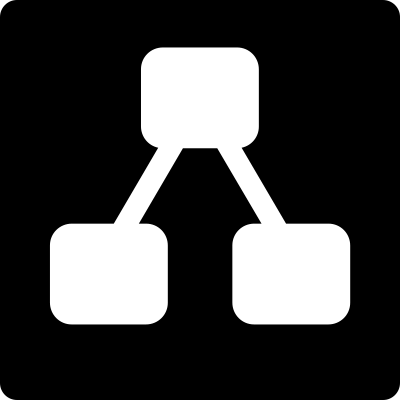
\includegraphics[width=0.30\textwidth]{images/drawio.png}
  \caption{Logo de draw.io (diagrams.net)}
\end{figure}
\noindent
draw.io (diagrams.net) est un outil de diagramme open source permettant de
réaliser les diagrammes UML, les schémas d'architecture et les modèles de base
de données. Il a servi à concevoir les diagrammes de cas d'utilisation, de
classes et l'architecture de l'application.~\cite{drawio}

\paragraph{3) Administration de la base de données :}
\begin{figure}[H]
  \centering
  
\includegraphics[width=0.30\textwidth]{images/prisma-studio.png}
  \caption{Logo de Prisma Studio}
\end{figure}
\noindent
Prisma Studio est une interface graphique fournie avec l'ORM Prisma. Elle permet
de visualiser et d'éditer les données de la base PostgreSQL directement depuis le
navigateur, ainsi que d'inspecter les relations entre les 44 modèles du schéma.~\cite{prisma}

\paragraph{4) Système de gestion de base de données :}
\begin{figure}[H]
  \centering
  
\includegraphics[width=0.30\textwidth]{images/postgresql.png}
  \caption{Logo de PostgreSQL}
\end{figure}
\noindent
PostgreSQL est un système de gestion de bases de données relationnelles
(SGBDR) open source, réputé pour sa robustesse, sa conformité au standard SQL
et son extensibilité. NeoLeadge utilise PostgreSQL~16 comme base de données
principale.~\cite{postgresql}

\begin{figure}[H]
  \centering
  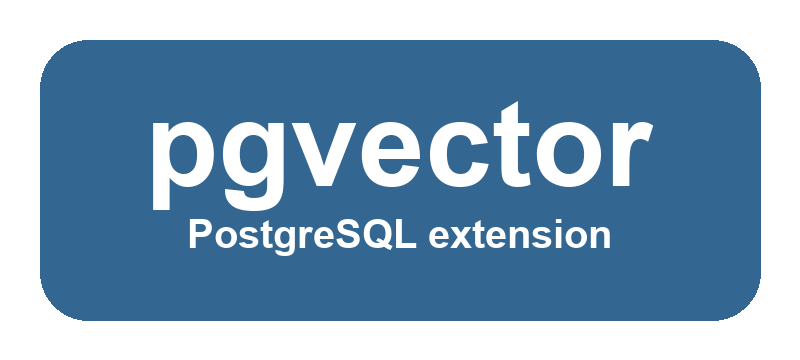
\includegraphics[width=0.30\textwidth]{images/pgvector.png}
  \caption{Logo de pgvector}
\end{figure}
\noindent
pgvector est une extension de PostgreSQL qui ajoute un type de données
\texttt{vector} et des index de similarité (HNSW). Elle est utilisée par
NeoLeadge pour la recherche sémantique : les transcriptions de réunions et les
réponses du questionnaire sont indexées sous forme de vecteurs (embeddings
\texttt{multilingual-e5-small}, 384 dimensions) afin que l'IA retrouve les
passages les plus pertinents lors de la génération du cahier des charges.~\cite{pgvector}

\paragraph{5) Conteneurisation et déploiement local :}
\begin{figure}[H]
  \centering
  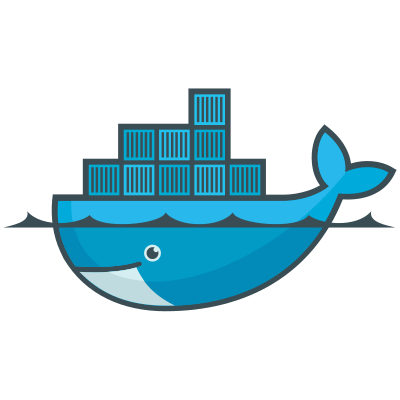
\includegraphics[width=0.30\textwidth]{images/docker.png}
  \caption{Logo de Docker}
\end{figure}
\noindent
Docker est une plateforme de conteneurisation qui permet d'empaqueter une
application et ses dépendances dans des conteneurs isolés. Avec Docker Compose,
l'ensemble de la stack NeoLeadge (serveur NestJS, frontend, base PostgreSQL,
service de transcription Python, reverse proxy Caddy) est orchestré et démarré
de façon reproductible aussi bien en local qu'en production.~\cite{docker}

\paragraph{6) Outil de réalisation du rapport :}
\begin{figure}[H]
  \centering
  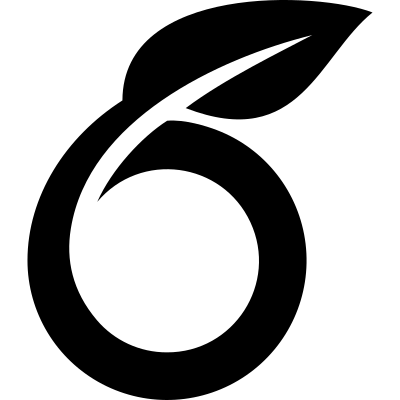
\includegraphics[width=0.30\textwidth]{images/overleaf.png}
  \caption{Logo d'Overleaf}
\end{figure}
\noindent
Overleaf est une plateforme web gratuite qui permet de créer et de modifier des
documents \LaTeX{} directement en ligne, sans installation, avec des
fonctionnalités de travail collaboratif sur un même document.~\cite{overleaf}

\begin{figure}[H]
  \centering
  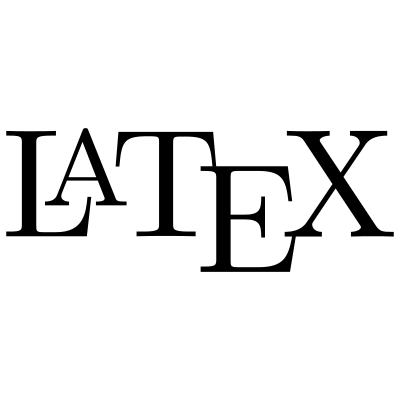
\includegraphics[width=0.25\textwidth]{images/latex.png}
  \caption{Logo de \LaTeX{}}
\end{figure}
\noindent
\LaTeX{} est un langage et un système de mise en forme de documents, constitué
d'un ensemble de macro-commandes conçues pour simplifier la production de
documents structurés de qualité professionnelle.~\cite{latex}

% ============================================================================
\section{Les langages de programmation et frameworks}

\subsection{Langages de programmation}

\begin{figure}[H]
  \centering
  
\includegraphics[width=0.28\textwidth]{images/typescript.png}
  \caption{Logo de TypeScript}
\end{figure}
\noindent
TypeScript est un sur-ensemble typé de JavaScript développé par Microsoft. Il
ajoute un système de types statiques qui sécurise le code et facilite la
maintenance. NeoLeadge est écrit intégralement en TypeScript, côté serveur
(NestJS) comme côté client (Vue~3).~\cite{typescript}

\begin{figure}[H]
  \centering
  
\includegraphics[width=0.18\textwidth]{images/html5.png}
  \caption{Logo de HTML5}
\end{figure}
\noindent
HTML est un langage de balisage utilisé pour créer et structurer les pages web.
Il permet d'écrire de l'hypertexte tout en définissant la structure sémantique
du contenu d'une page.~\cite{html}

\begin{figure}[H]
  \centering
  
\includegraphics[width=0.18\textwidth]{images/css3.png}
  \caption{Logo de CSS3}
\end{figure}
\noindent
Le CSS est un langage utilisé pour styliser les pages HTML. Il sépare le contenu
de la mise en forme. Dans NeoLeadge, le style s'appuie sur Tailwind CSS et sur
les composants de la bibliothèque NeoLibrary.~\cite{css}

\begin{figure}[H]
  \centering
  
\includegraphics[width=0.22\textwidth]{images/python.png}
  \caption{Logo de Python}
\end{figure}
\noindent
Python est un langage de haut niveau réputé pour sa lisibilité et son riche
écosystème scientifique. Il est utilisé pour le microservice de transcription
NeoLeadge (FastAPI + faster-whisper + SpeechBrain) et pour le service
d'embeddings sémantiques.~\cite{python}

\subsection{Les frameworks et bibliothèques}

\begin{figure}[H]
  \centering
  
\includegraphics[width=0.30\textwidth]{images/nodejs.png}
  \caption{Logo de Node.js}
\end{figure}
\noindent
Node.js est un environnement d'exécution JavaScript côté serveur, basé sur le
moteur V8 de Chrome. Son fonctionnement asynchrone et son écosystème npm en font
une base efficace pour les API REST. Le serveur NeoLeadge s'exécute sur Node.js.~\cite{nodejs}

\begin{figure}[H]
  \centering
  
\includegraphics[width=0.30\textwidth]{images/nestjs.png}
  \caption{Logo de NestJS}
\end{figure}
\noindent
NestJS est un framework Node.js progressif pour construire des applications
serveur efficaces et maintenables. Il s'appuie sur TypeScript et une
architecture modulaire (modules, contrôleurs, services, injection de
dépendances). NeoLeadge utilise NestJS~11 pour son API REST, ses WebSockets
(Socket.IO) et ses tâches planifiées.~\cite{nestjs}

\begin{figure}[H]
  \centering
  
\includegraphics[width=0.30\textwidth]{images/vue.png}
  \caption{Logo de Vue.js}
\end{figure}
\noindent
Vue.js est un framework JavaScript progressif open source utilisé pour
construire des interfaces utilisateur et des applications monopages (SPA). La
version~3 introduit la Composition API et un système de réactivité performant.
NeoLeadge utilise Vue~3 pour l'ensemble de son interface.~\cite{vue}

\begin{figure}[H]
  \centering
  
\includegraphics[width=0.28\textwidth]{images/vite.png}
  \caption{Logo de Vite}
\end{figure}
\noindent
Vite est un outil de build et un serveur de développement nouvelle génération.
Il offre un démarrage quasi instantané et un rechargement à chaud (HMR) rapide
grâce aux modules ES natifs. Il sert de bundler au frontend NeoLeadge.~\cite{vite}

\begin{figure}[H]
  \centering
  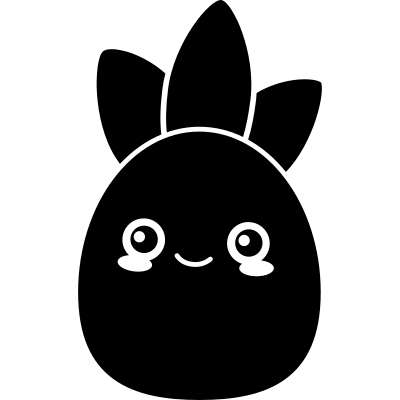
\includegraphics[width=0.24\textwidth]{images/pinia.png}
  \caption{Logo de Pinia}
\end{figure}
\noindent
Pinia est la bibliothèque officielle de gestion d'état pour Vue~3. Elle centralise
l'état partagé de l'application (utilisateur, projets, notifications) de manière
typée et réactive.~\cite{pinia}

\begin{figure}[H]
  \centering
  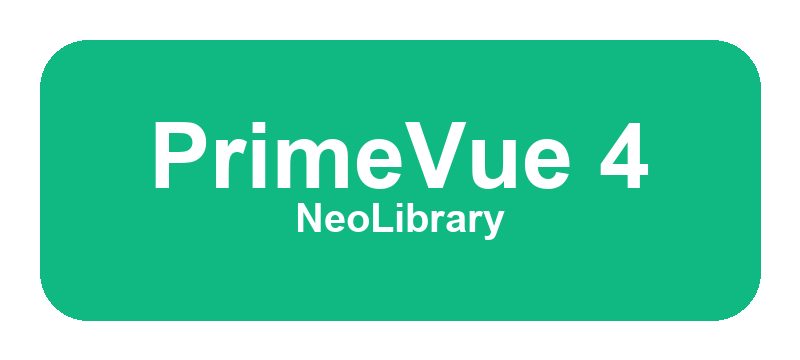
\includegraphics[width=0.30\textwidth]{images/primevue.png}
  \caption{Logo de PrimeVue / NeoLibrary}
\end{figure}
\noindent
NeoLibrary est la bibliothèque de composants interne du projet, construite
au-dessus de PrimeVue~4 (boutons, tableaux, formulaires, fenêtres modales,
calendriers) avec un style Tailwind personnalisé. Elle garantit une interface
cohérente sur l'ensemble de l'application.~\cite{primevue}

\begin{figure}[H]
  \centering
  
\includegraphics[width=0.28\textwidth]{images/prisma-studio.png}
  \caption{Logo de Prisma}
\end{figure}
\noindent
Prisma est un ORM (mapping objet-relationnel) moderne pour TypeScript. Il génère
un client typé à partir d'un schéma déclaratif, gère les migrations versionnées
et sécurise les requêtes. NeoLeadge utilise Prisma~7 avec l'adaptateur
\texttt{@prisma/adapter-pg} pour PostgreSQL.~\cite{prisma}

\begin{figure}[H]
  \centering
  
\includegraphics[width=0.30\textwidth]{images/fastapi.png}
  \caption{Logo de FastAPI}
\end{figure}
\noindent
FastAPI est un framework web Python rapide et moderne pour construire des API.
NeoLeadge l'utilise pour son microservice de transcription audio
(faster-whisper + SpeechBrain) et son point d'accès d'embeddings sémantiques.~\cite{fastapi}

\begin{figure}[H]
  \centering
  
\includegraphics[width=0.28\textwidth]{images/socketio.png}
  \caption{Logo de Socket.IO}
\end{figure}
\noindent
Socket.IO permet une communication bidirectionnelle en temps réel entre le
serveur et les clients. NeoLeadge l'utilise pour les notifications instantanées
et la présence collaborative pendant l'édition des questionnaires.~\cite{socketio}

\subsection{Autres logiciels et services}

\begin{figure}[H]
  \centering
  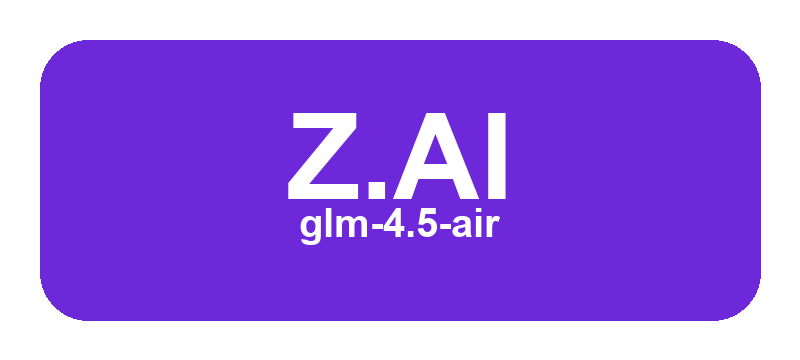
\includegraphics[width=0.28\textwidth]{images/zai.png}
  \caption{Logo de Z.AI}
\end{figure}
\noindent
Z.AI fournit le modèle de langage \texttt{glm-4.5-air} (compatible avec l'API
OpenAI) utilisé par NeoLeadge pour l'ensemble des fonctionnalités d'IA :
analyse des réunions, génération du cahier des charges, proposition de backlog
et suggestions d'affectation des tâches.~\cite{zai}

\begin{figure}[H]
  \centering
  
\includegraphics[width=0.28\textwidth]{images/postman.png}
  \caption{Logo de Postman}
\end{figure}
\noindent
Postman est une application qui permet de tester et d'explorer les API de manière
simple et efficace, et de partager les tests entre développeurs.~\cite{postman}

\begin{figure}[H]
  \centering
  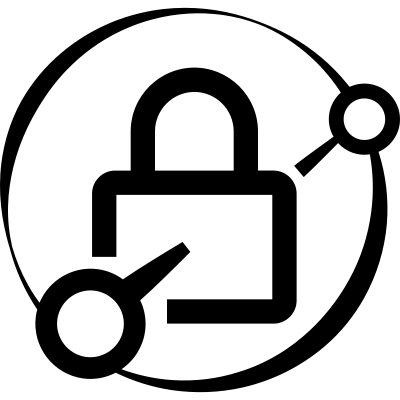
\includegraphics[width=0.28\textwidth]{images/caddy.png}
  \caption{Logo de Caddy}
\end{figure}
\noindent
Caddy est un serveur web et reverse proxy qui gère automatiquement les
certificats TLS via Let's Encrypt. En production, il route le trafic HTTPS vers
le frontend et l'API NeoLeadge sur \texttt{https://neoleadge.pythagore-init.com}.~\cite{caddy}

\begin{figure}[H]
  \centering
  
\includegraphics[width=0.22\textwidth]{images/github.png}
  \caption{Logo de GitHub}
\end{figure}
\noindent
GitHub est une plateforme en ligne qui permet d'héberger, de gérer et de
collaborer sur des projets utilisant le système de gestion de versions Git. Le
dépôt NeoLeadge y est hébergé, avec une intégration continue (GitHub Actions)
qui exécute les tests à chaque \textit{pull request}.~\cite{github}

% ============================================================================
\section{Architecture de projet}

\subsection{L'architecture logicielle utilisée}

NeoLeadge repose sur une \textbf{architecture en couches modulaire} côté serveur
(NestJS) et sur une architecture de composants côté client (Vue~3). Côté serveur,
chaque domaine fonctionnel est isolé dans un module dédié, structuré en trois
responsabilités distinctes :

\begin{itemize}
  \item \textbf{Contrôleur (Controller)} \\
  \textit{Rôle :} il reçoit les requêtes HTTP, valide les données entrantes
  (DTO + \texttt{ValidationPipe}) et délègue le traitement au service approprié,
  puis transforme le résultat en réponse HTTP.
  \item \textbf{Service (Service)} \\
  \textit{Rôle :} il porte la logique métier. Chaque méthode retourne un objet
  \texttt{Result.ok} ou \texttt{Result.fail} plutôt que de lever une exception,
  ce qui rend la gestion d'erreurs explicite et prévisible.
  \item \textbf{Accès aux données (Prisma)} \\
  \textit{Rôle :} la couche d'accès aux données s'appuie sur l'ORM Prisma, qui
  encapsule les requêtes vers PostgreSQL et garantit un typage de bout en bout.
\end{itemize}

\noindent
Côté client, Vue~3 organise l'interface en composants réutilisables, l'état
partagé étant géré par Pinia. La séparation des responsabilités y reste claire :
vues (pages), composants, magasins (stores) et services d'accès à l'API.

\begin{figure}[H]
  \centering
  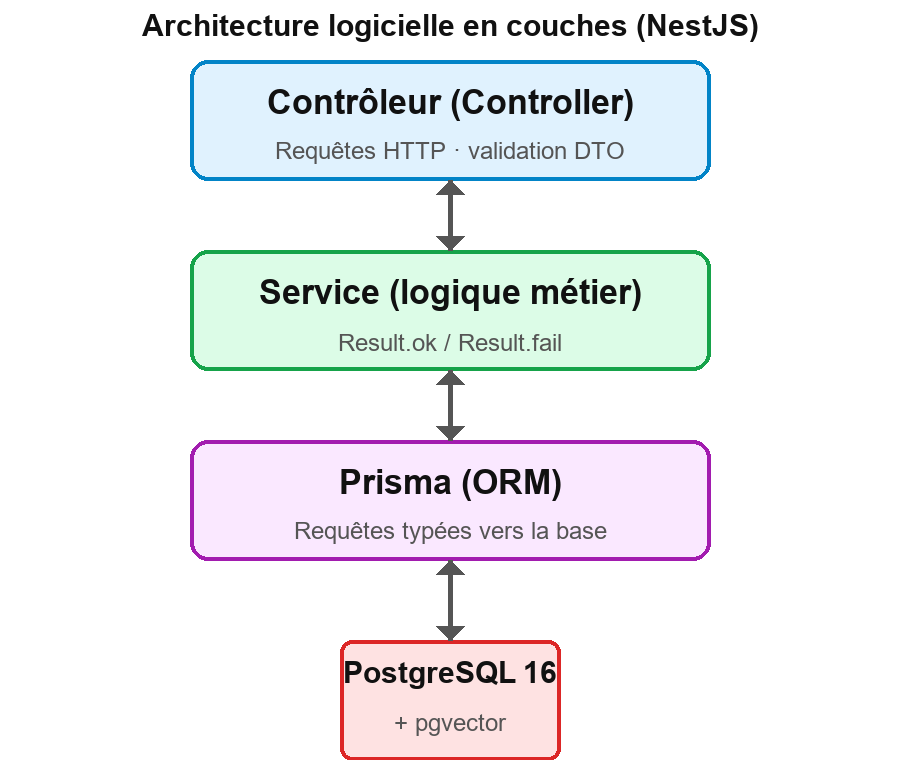
\includegraphics[width=0.70\textwidth]{images/archi-couches.png}
  \caption{Architecture logicielle en couches (NestJS)}
\end{figure}

\subsection{Architecture physique}

Cette partie présente l'architecture physique de l'application et les
technologies déployées. L'application est construite autour de plusieurs services
conteneurisés orchestrés par Docker Compose.

\begin{figure}[H]
  \centering
  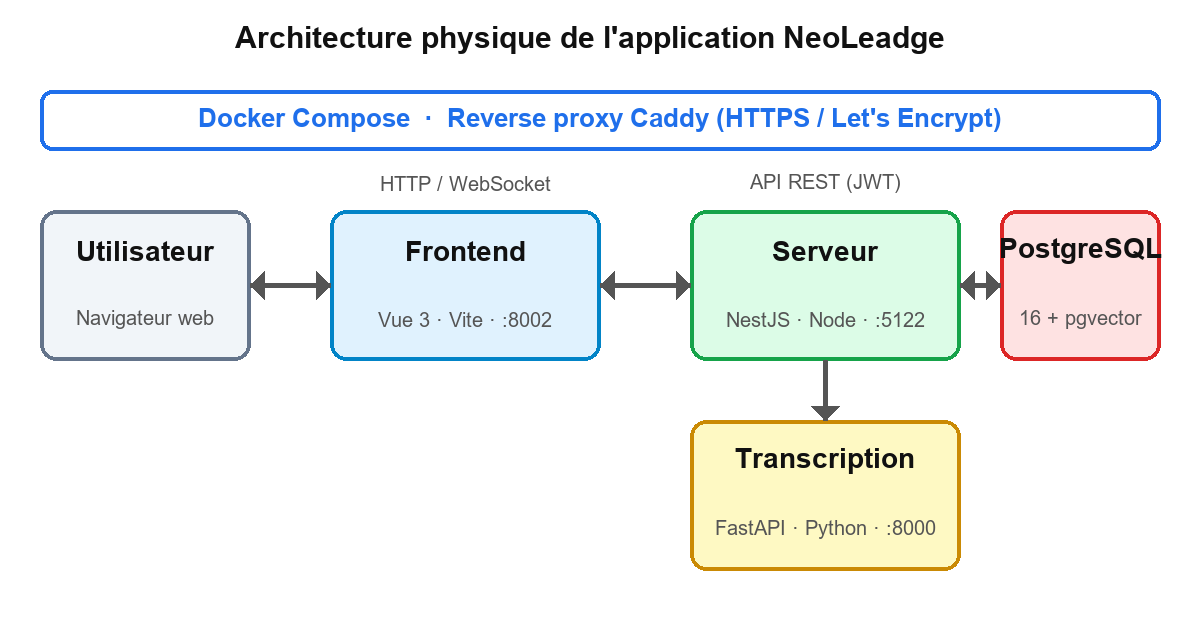
\includegraphics[width=0.80\textwidth]{images/archi-physique.png}
  \caption{Architecture physique de l'application NeoLeadge}
\end{figure}

\noindent
L'architecture physique se compose des éléments suivants :

\paragraph{Côté client (Vue 3 + Vite) :}
\begin{itemize}
  \item Application monopage (SPA) servie en production par un conteneur web
  (port 8002) derrière le reverse proxy Caddy.
  \item Communication avec l'API via des requêtes HTTP (axios) et des WebSockets
  (Socket.IO) pour le temps réel.
\end{itemize}

\paragraph{Côté serveur (NestJS sur Node.js, port 5122) :}
\begin{itemize}
  \item Gestion et traitement des requêtes HTTP entrantes (API REST sécurisée
  par JWT).
  \item Connexion et manipulation des données via Prisma vers PostgreSQL.
  \item Gestion des opérations asynchrones et des tâches planifiées (analyse IA
  des réunions, échéances, rétention).
\end{itemize}

\paragraph{Base de données (PostgreSQL 16 + pgvector) :}
\begin{itemize}
  \item Stockage relationnel des données métier (44 modèles).
  \item Recherche sémantique vectorielle (index HNSW) pour les fonctionnalités
  d'IA.
\end{itemize}

\paragraph{Service de transcription (Python / FastAPI, port 8000) :}
\begin{itemize}
  \item Transcription audio des réunions (faster-whisper) et diarisation des
  locuteurs (SpeechBrain).
  \item Génération des embeddings sémantiques (\texttt{multilingual-e5-small}).
\end{itemize}

\paragraph{Orchestration et déploiement :}
\begin{itemize}
  \item L'ensemble des services est défini dans un fichier Docker Compose et
  déployé sur un serveur Linux.
  \item Le reverse proxy Caddy assure la terminaison TLS (Let's Encrypt) et le
  routage HTTPS vers le frontend et l'API.
\end{itemize}
